\noindent Beyond the data collection pipelines used in the main text and Appendix~\ref{appendix:pipeline}, we explored alternative data sources for neural-computer prototyping.
These routes were not incorporated into the final pipeline, but the trials yielded useful insights and suggest directions for future work as tooling matures and data-collection infrastructure scales.

\begin{figure}[h]
  \centering
  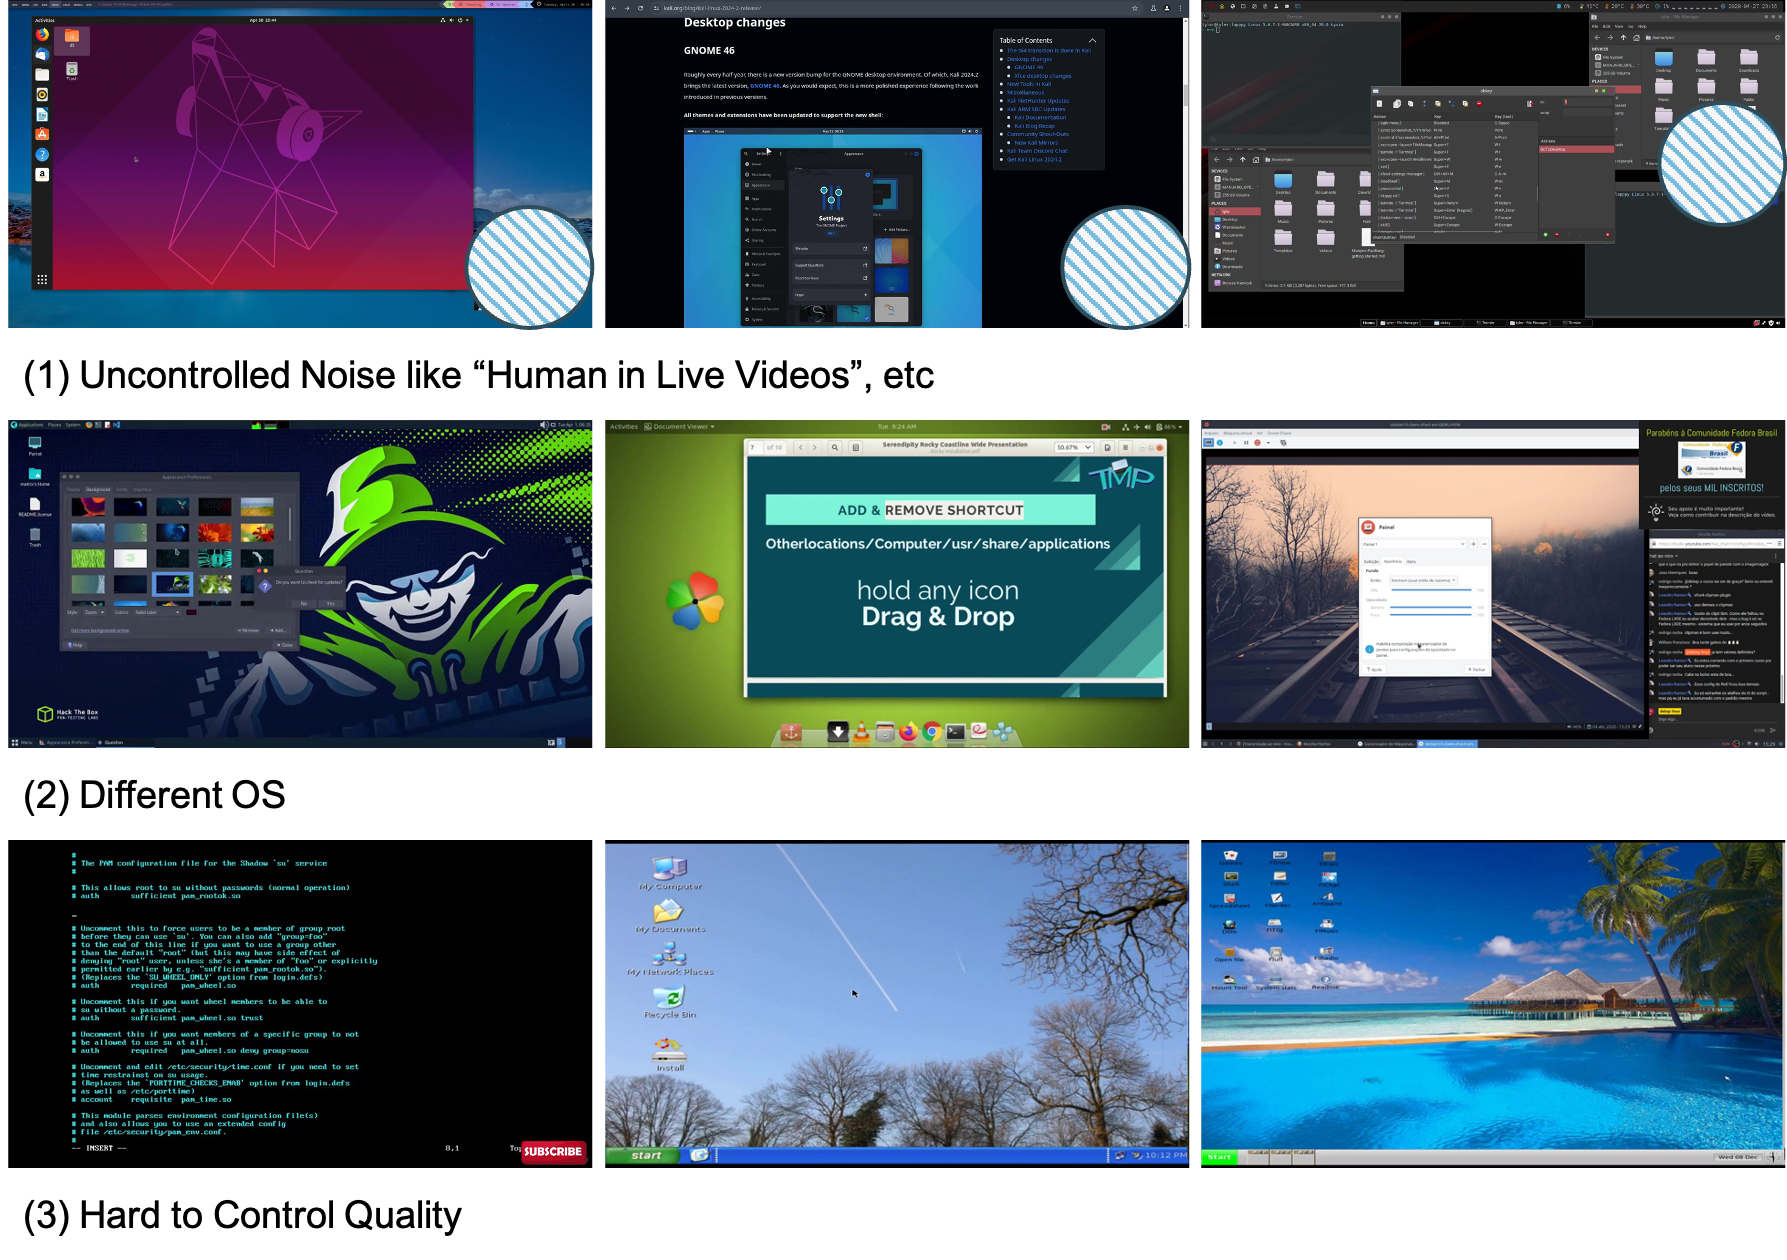
\includegraphics[width=\linewidth]{assets/web_data_issue.png}
  \vspace{-0.4em}
  \caption{\textbf{Common issues in web-scale screen video crawling.}
  Web videos mix uncontrolled content, heterogeneous OS/UI configurations, and inconsistent capture quality.
  This makes terminal localization, OCR, and time alignment unreliable without heavy filtering and sanitization.}
  \vspace{-10pt}
  \label{fig:web-video-issues}
\end{figure}

\subsection{Web video extraction}
We initially tested crawling computer-use videos from the web.
We used OCR and layout detectors to locate terminal regions, estimate text content and timestamps, and extract related clips.
We did not adopt this route for two main reasons:
\begin{tcolorbox}[
  colback=metablue!8,
  colframe=metablue!40,
  boxrule=0pt,
  borderline west={1pt}{0pt}{gray!60},
  left=6pt,right=4pt,top=3pt,bottom=3pt]
\small
\begin{itemize}
  \setlength{\itemsep}{2pt}
  \setlength{\topsep}{2pt}
  \item \textbf{Data governance constraints:} privacy and copyright risks are difficult to manage at web scale.
  \item \textbf{Data quality burden:} heavy filtering and sanitization are required before the data can support reliable OCR and temporal alignment.
\end{itemize}
\end{tcolorbox}
Screen recordings can contain personal identifiers (usernames, emails, file paths, chat content) and may come with licensing constraints that are difficult to verify at scale.
Cleaning the resulting data is substantially more complex than it appears (Figure~\ref{fig:web-video-issues}).
Typical failure modes include (i) uncontrolled content such as faces/hands, picture-in-picture overlays, and unrelated desktop activity;
(ii) domain shift across operating systems, themes, fonts, resolutions, and window managers; and
(iii) quality factors such as compression artifacts, variable frame rates, zoom/crop edits, and inconsistent capture pipelines.
These factors degrade OCR and temporal alignment.



Despite these challenges, web videos remain a potential long-term scaling axis for interface experience.
In this work, however, the cost--quality trade-off was unfavorable.
Our setting benefits disproportionately from clean, temporally aligned text and interaction signals.
Building a high-precision web filter also requires substantial upfront investment.
This includes rights-cleared sourcing or licensing, privacy review and redaction, and large-scale multimodal filtering/OCR pipelines that often rely on paid APIs.
Given these constraints and our emphasis on high-quality supervision, we prioritized curated, rights-cleared interface trajectories.
Future efforts that invest in rights-respecting acquisition and stronger automated filtering could unlock web-scale data as a complementary scaling axis.

\subsection{Online environment interaction}
We prototyped an agentic interaction pipeline that separates a control plane from an execution environment plane (Figure~\ref{fig:online-interaction-pipeline}).
In the environment plane, a sandboxed container runs a live shell together with LLM agents (planner/controller) and a recorder exposed via a narrow port-based interface.
The agents issue commands and control actions.
The recorder captures synchronized terminal renders, structured terminal state when available (e.g., buffer/text), and action traces.
Structured terminal state is logged for diagnostics/alignment and is not fed to video models as privileged state input.
Trajectories are streamed to the control plane for storage and video-model updates.

\begin{figure}[h]
  \centering
  \includesvg[inkscapelatex=false,width=\linewidth]{agentic_online_training}
  \vspace{-1.4em}
  \caption{\textbf{Agentic online interaction pipeline (early exploration).}
  A control plane ingests trajectories for storage and video-model updates (online where feasible, with offline replay support).
  A sandboxed environment plane executes an agent in an isolated container and records synchronized state/action traces.}
  \vspace{-10pt}
  \label{fig:online-interaction-pipeline}
\end{figure}


Concretely, the environment plane exposes a minimal ``step/reset'' interface over a port.
It returns multimodal observations that can be logged deterministically (rendered screenshots plus structured state when available).
The agent emits structured actions (typed command text, key/mouse events when applicable, and timing).
This separation makes rollouts auditable and lets the control plane scale rollout collection and model updates with decoupled throughput.

We explored this setup because closed-loop interaction can induce a natural curriculum by continually sampling the boundary of current video-model behavior.
It can also surface rare and safety-critical failure modes that do not appear in offline logs.
It supports targeted data collection (e.g., focusing on specific tools, error recovery, or long-horizon tasks).
In principle, it also offers a direct path to scaling \emph{experience} rather than only scaling static demonstrations.

Early trials showed promise, but the dominant bottlenecks in the end-to-end system were systems-level: cross-cluster communication latency between rollout workers and training nodes, and high debugging complexity in asynchronous distributed execution.
Safety controls (e.g., isolation of untrusted code execution, monitoring and abuse prevention, and deterministic resets and environment control) remained necessary constraints, but they were not the primary bottleneck.
The setup also requires robust recording and serialization across heterogeneous environments.
Under time and cost constraints, we therefore prioritized controlled video data for the main experiments. 
Despite not being used in the final pipeline, we consider this design a useful systems template for future work.
It supports scalable multi-environment rollout collection and consistent provenance and storage of trajectories.
It can support multiple downstream learning algorithms (e.g., behavior cloning or preference-based learning).
Execution remains sandboxed and auditable.
